% !TeX root = ../main.tex
\section{Results}
\label{sec:results}

% --------------------------------------------------------
\subsection{Sentinel-1 backscatter responses to harvest events}
\label{sec:s1_signatures}

Across the 978 reference harvest events meeting the paired VV--VH coverage requirements, harvesting consistently reduced C-band backscatter in both polarizations, even though pooled pre- and post-harvest backscatter distributions overlapped substantially (Fig.~\ref{fig:s1_population_signatures}a). Median VV backscatter declined from $-6.00$~dB before harvesting (months $-12$ to $-3$) to $-7.51$~dB immediately afterward (months $0$ to $+2$), while median VH declined from $-12.54$ to $-13.98$~dB. Within individual stands, however, paired post-minus-pre changes were negative in 97.3\% of events for VV and 95.0\% for VH, with median declines of $-1.45$~dB (95\% CI: $-1.64$ to $-1.24$~dB) and $-1.40$~dB (95\% CI: $-1.60$ to $-1.19$~dB), respectively (Fig.~\ref{fig:s1_population_signatures}b).

\begin{figure*}[pos=!htbp]
    \centering
    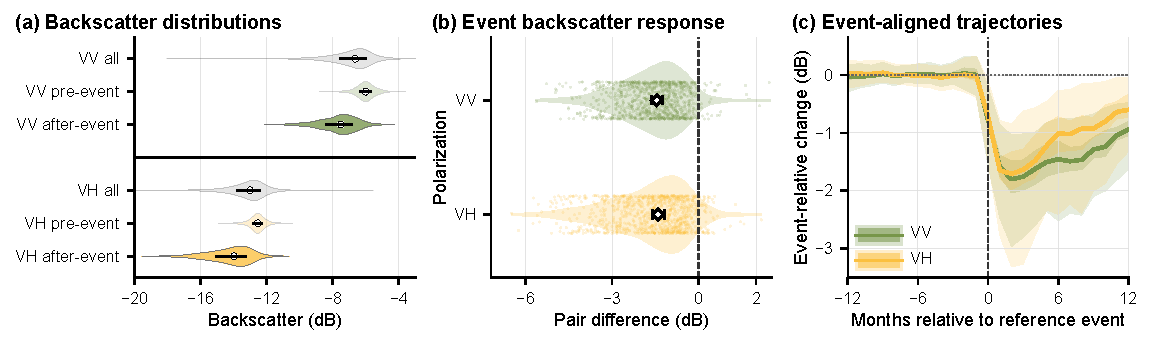
\includegraphics[width=\linewidth]{figures/fig05_backscatter_signatures.pdf}
    \caption{Sentinel-1 VV and VH backscatter responses across 978 reference harvests. (a) Pre-event ($-12$ to $-3$ months), after-event ($0$ to $+2$ months), and inventory-wide (all) monthly backscatter distributions (medians and IQRs). (b) Paired post-minus-pre differences within events (medians and 95\% CIs). (c) Event-aligned relative backscatter trajectories with IQRs (light shading) and 95\% spatial-block bootstrap CIs (dark shading).}
    \label{fig:s1_population_signatures}
\end{figure*}

Event-aligned trajectories showed sharp backscatter drops at harvesting followed by gradual recovery during early stand regrowth (Fig.~\ref{fig:s1_population_signatures}c). Median deviations reached their minimum at month $+2$ ($-1.80$~dB for VV and $-1.71$~dB for VH) and subsequently converged toward pre-harvest baselines. Across the 950 events with complete 12-month post-harvest coverage, median deviations remained negative at month $+12$ ($-0.94$~dB for VV and $-0.60$~dB for VH), with pointwise 95\% confidence intervals remaining below zero from month $0$ through month $+12$ in both polarizations.

% --------------------------------------------------------
\subsection{Component contributions and configuration sensitivity}
\label{sec:cusum_components_sensitivity}

\subsubsection{Contributions of local context and candidate screening}
\label{sec:representation_component_ablation}

Progressive component ablation demonstrated that local context windows provide the sensitivity needed to capture repeated harvests, whereas central decision-interval admission and permutation testing establish precision (Table~\ref{tab:component_ablation}). Evaluating each pixel trajectory with a single full-record CuSum yielded high precision ($0.810$) but missed nearly half of all documented harvests ($R_{\mathrm{ref}}=0.531$, $F_{1,\mathrm{ref}}=0.641$), recovering only 18.0\% (106/590) of chronologically adjacent reference harvest pairs. Replacing the full-record baseline with overlapping 36-month local windows raised recall to $0.952$ (999/1,049 events) and adjacent-pair recovery to 93.4\% (551/590), but unscreened repeated searches inflated stand-level detected events from 688 to 2,327, lowering precision to $0.429$ ($\Delta F_{1,\mathrm{ref}}=-0.050$).

\begin{table*}[pos=!htbp]
    \centering
    \small
    \setlength{\tabcolsep}{4pt}
    \caption{Progressive component ablation of windowed CuSum across 459 reference stands (1,049 harvests). $N_{\mathrm{det}}$ and $M$ denote detected stand-level events and matched harvests; $\Delta F_{1,\mathrm{ref}}$ compares each row with its predecessor (95\% bootstrap CIs). Bold marks column maxima.}
    \label{tab:component_ablation}
    \begin{tabular*}{\linewidth}{@{\extracolsep{\fill}}lrrrrrc@{}}
        \toprule
        Cumulative configuration &
        $N_{\mathrm{det}}$ &
        $M$ &
        $P_{\mathrm{ref}}$ &
        $R_{\mathrm{ref}}$ &
        $F_{1,\mathrm{ref}}$ &
        $\Delta F_{1,\mathrm{ref}}$ (95\% CI) \\
        \midrule
        Full-record CuSum
        & 688 & 557 & \textbf{0.810} & 0.531 & 0.641 & -- \\
        + Local windows
        & 2,327 & 999 & 0.429 & \textbf{0.952} & 0.592 & $-0.050$ [$-0.075$, $-0.022$] \\
        + Decision-interval admission
        & 1,843 & 992 & 0.538 & 0.946 & 0.686 & $+0.094$ [$+0.081$, $+0.107$] \\
        + Negative-direction screening
        & 1,843 & 992 & 0.538 & 0.946 & 0.686 & $\phantom{+}0.000$ [$\phantom{+}0.000$, $\phantom{+}0.000$] \\
        + Permutation screening
        & 1,208 & 945 & 0.782 & 0.901 & \textbf{0.837} & $+0.151$ [$+0.134$, $+0.169$] \\
        \bottomrule
    \end{tabular*}
\end{table*}

Restricting candidate admission to the central 12-month decision interval eliminated 484 boundary-induced events while forfeiting only seven matched harvests, lifting $F_{1,\mathrm{ref}}$ to $0.686$ ($\Delta F_{1,\mathrm{ref}}=+0.094$). Because localizing candidates at the global cumulative residual maximum already selected downward shifts across all 79,301 admitted pixel--month candidates, explicit negative-direction screening left detections unchanged ($\Delta F_{1,\mathrm{ref}}=0.000$). Finally, window-specific permutation testing ($\alpha_{\mathrm{ts}}=0.025$) removed 635 low-confidence events while retaining 945 matched harvests, raising precision to $0.782$ and $F_{1,\mathrm{ref}}$ to $0.837$ ($\Delta F_{1,\mathrm{ref}}=+0.151$). The complete configuration recovered 83.9\% (495/590) of adjacent reference pairs and produced compact stand-level events with a median detection span of four months (with 6.4\%, or 77 events, exceeding 12 months).

\subsubsection{Configuration sensitivity of windowed CuSum}
\label{sec:cusum_configuration_sensitivity}

Detection performance remained stable across moderate variations in window length and search schedule, while showing clear sensitivity to polarization choice and block-permutation length (Table~\ref{tab:cusum_configuration_sensitivity}). Shortening the context window to $W=24$ months slightly increased precision ($0.808$) and yielded an $F_{1,\mathrm{ref}}$ of $0.848$ ($\Delta F_{1,\mathrm{ref}}=+0.010$, 95\% CI: $-0.004$ to $+0.025$), though with fewer matched harvests (935 vs.\ 945) and adjacent pairs (486/590 vs.\ 495/590) than the $W=36$ baseline. Conversely, extending the window to $W=48$ and $W=60$ months progressively reduced recall ($0.860$ and $0.823$) and adjacent-pair recovery (452/590 and 407/590), lowering $F_{1,\mathrm{ref}}$ to $0.820$ at $W=60$ ($\Delta F_{1,\mathrm{ref}}=-0.017$). Halving the search stride ($D=12, S=6$) or both interval and stride ($D=S=6$) produced $F_{1,\mathrm{ref}}$ values nearly indistinguishable from the annual baseline ($0.834$ and $0.840$; paired differences within $\pm0.004$, with 95\% CIs spanning zero), recovering 518/590 and 487/590 adjacent pairs with median event spans of five and four months, respectively. Combining $W=24$ with $D=S=6$ similarly yielded $F_{1,\mathrm{ref}}=0.843$ ($\Delta F_{1,\mathrm{ref}}=+0.005$, 95\% CI: $-0.007$ to $+0.018$).

\begin{table*}[pos=!htbp]
    \centering\small
    \setlength{\tabcolsep}{3pt}
    \caption{Configuration sensitivity of windowed CuSum relative to the baseline (VV, $W=36$, $D=S=12$ months, $\alpha_{\mathrm{ts}}=0.025$). $\Delta F_{1,\mathrm{ref}}$ shows differences from baseline (95\% bootstrap CIs). Bold marks column maxima.}
    \label{tab:cusum_configuration_sensitivity}
    \begin{tabular*}{\linewidth}{@{\extracolsep{\fill}}lrrrrrc@{}}
        \toprule
        Configuration & $N_{\mathrm{det}}$ & $M$ & $P_{\mathrm{ref}}$ & $R_{\mathrm{ref}}$ & $F_{1,\mathrm{ref}}$ & $\Delta F_{1,\mathrm{ref}}$ (95\% CI) \\
        \midrule
        Baseline ($W=36$, $D=S=12$, VV) & 1,208 & 945 & 0.782 & 0.901 & 0.837 & -- \\
        \midrule
        \multicolumn{7}{@{}l}{\textit{Context length ($D=S=12$)}} \\
        $W=24$ months & 1,157 & 935 & 0.808 & 0.891 & \textbf{0.848} & $+0.010$ [$-0.004$, $+0.025$] \\
        $W=48$ months & 1,120 & 902 & 0.805 & 0.860 & 0.832 & $-0.006$ [$-0.018$, $+0.006$] \\
        $W=60$ months & 1,056 & 863 & 0.817 & 0.823 & 0.820 & $-0.017$ [$-0.033$, $-0.002$] \\
        \midrule
        \multicolumn{7}{@{}l}{\textit{Search schedule ($W=36$)}} \\
        $D=12$, $S=6$ months & 1,273 & 968 & 0.760 & 0.923 & 0.834 & $-0.004$ [$-0.011$, $+0.005$] \\
        $D=S=6$ months & 1,188 & 940 & 0.791 & 0.896 & 0.840 & $+0.003$ [$-0.006$, $+0.012$] \\
        \midrule
        \multicolumn{7}{@{}l}{\textit{Polarization ($W=36$, $D=S=12$)}} \\
        VH & 1,127 & 852 & 0.756 & 0.812 & 0.783 & $-0.054$ [$-0.072$, $-0.036$] \\
        VV--VH union & 1,430 & 976 & 0.683 & \textbf{0.930} & 0.787 & $-0.050$ [$-0.061$, $-0.038$] \\
        VV--VH intersection & 809 & 737 & \textbf{0.911} & 0.703 & 0.793 & $-0.044$ [$-0.064$, $-0.025$] \\
        \bottomrule
    \end{tabular*}
\end{table*}

Among polarization strategies, VV alone outperformed VH ($F_{1,\mathrm{ref}}=0.783$, $\Delta F_{1,\mathrm{ref}}=-0.054$) as well as dual-polarization fusion: taking the VV--VH union raised recall to $0.930$ at the expense of precision ($0.683$, $F_{1,\mathrm{ref}}=0.787$; and $0.807$ vs.\ $0.843$ under $W=24, D=S=6$), whereas requiring $\pm2$-month VV--VH agreement raised precision to $0.911$ but depressed recall to $0.703$ ($F_{1,\mathrm{ref}}=0.793$). Varying the permutation threshold across $\alpha_{\mathrm{ts}}\in[0.005,0.10]$ kept $F_{1,\mathrm{ref}}$ within $0.804\text{--}0.847$, peaking at $\alpha_{\mathrm{ts}}=0.01$ ($\Delta F_{1,\mathrm{ref}}=+0.009$, 95\% CI: $-0.001$ to $+0.019$). In contrast, replacing independent shuffling with calendar-block permutations of 3, 4, 5, and 6 months sharply curtailed sensitivity within the 36-month window, reducing recall to $0.647$, $0.397$, $0.090$, and $0.015$ and $F_{1,\mathrm{ref}}$ to $0.744$, $0.550$, $0.163$, and $0.030$, respectively.

% --------------------------------------------------------
\subsection{Benchmark performance against alternative detectors}
\label{sec:benchmark_null_sensitivity}

Windowed CuSum achieved the highest overall accuracy ($F_{1,\mathrm{ref}}=0.837$) among all 14 evaluated detector configurations (Table~\ref{tab:benchmark_comparison}). In the two primary Bonferroni-adjusted contrasts, windowed CuSum outperformed raw monthly CuSum NRT by $+0.253$ in $F_{1,\mathrm{ref}}$ (97.5\% CI: $0.230$ to $0.275$) and the original CCDC configuration by $+0.103$ (97.5\% CI: $0.076$ to $0.133$). Extreme operating points emerged among specialized alternatives: decrease-filtered monthly CuSum NRT achieved the highest recall ($0.939$, 985/1,049 events) but generated 1,960 stand-level events ($P_{\mathrm{ref}}=0.503$, $F_{1,\mathrm{ref}}=0.655$), with a median event span of seven months (and 32.6\% of events exceeding 12 months for raw NRT), whereas the dual-polarization BOCD prototype achieved the highest precision ($0.888$) at the cost of missing four-fifths of reference harvests ($R_{\mathrm{ref}}=0.197$).

\begin{table*}[pos=!htbp]
    \centering
    \small
    \setlength{\tabcolsep}{4pt}
    \caption{Benchmark comparison of 14 detector configurations across 459 reference stands (1,049 harvests) under identical TDA rules. Bold marks column maxima.}
    \label{tab:benchmark_comparison}
    \begin{tabular*}{\linewidth}{@{\extracolsep{\fill}}lrrrrr@{}}
        \toprule
        Detector configuration & $N_{\mathrm{det}}$ & $M$ & $P_{\mathrm{ref}}$ & $R_{\mathrm{ref}}$ & $F_{1,\mathrm{ref}}$ \\
        \midrule
        Windowed CuSum (Ours) & 1,208 & 945 & 0.782 & 0.901 & \textbf{0.837} \\
        Maximum monthly decline & 2,470 & 691 & 0.280 & 0.659 & 0.393 \\
        Classical lower CuSum & 1,254 & 317 & 0.253 & 0.302 & 0.275 \\
        BOCD prototype (VV+VH) & 233 & 207 & \textbf{0.888} & 0.197 & 0.323 \\
        Monthly CuSum NRT (raw) & 2,159 & 938 & 0.434 & 0.894 & 0.585 \\
        Monthly CuSum NRT (decrease-filtered) & 1,960 & 985 & 0.503 & \textbf{0.939} & 0.655 \\
        ReCuSum (decrease-filtered) & 946 & 763 & 0.807 & 0.727 & 0.765 \\
        ReCuSum (raw) & 1,688 & 716 & 0.424 & 0.683 & 0.523 \\
        ReCuSum first-post adaptation & 1,024 & 818 & 0.799 & 0.780 & 0.789 \\
        CCDC original configuration & 953 & 735 & 0.771 & 0.701 & 0.734 \\
        CCDC expanded configuration & 825 & 659 & 0.799 & 0.628 & 0.703 \\
        Structural breakpoints & 902 & 729 & 0.808 & 0.695 & 0.747 \\
        BFAST Monitor adaptation & 773 & 207 & 0.268 & 0.197 & 0.227 \\
        EWMACD adaptation & 1,135 & 473 & 0.417 & 0.451 & 0.433 \\
        \bottomrule
    \end{tabular*}
\end{table*}

The strongest external competitor was the first-post adaptation of recursive ReCuSum ($F_{1,\mathrm{ref}}=0.789$), over which windowed CuSum gained $+0.048$ in $F_{1,\mathrm{ref}}$ (95\% CI: $0.032$ to $0.065$). While both methods maintained comparable precision ($0.782$ vs.\ $0.799$), identical median event spans (four months; 6.4\% vs.\ 5.3\% exceeding 12 months), and virtually identical dating accuracy across 804 shared matches (representative-month MAE of $0.803$ vs.\ $0.799$ months; paired difference $+0.005$ months, 95\% CI: $-0.039$ to $+0.048$), windowed CuSum substantially improved multi-rotation completeness, lifting single-event recall from 78.0\% to 90.1\% and adjacent-pair recovery from 65.6\% (387/590) to 83.9\% (495/590).

% --------------------------------------------------------
\subsection{Mapping rotational harvesting across mainland Ecuador}
\label{sec:harvest_mapping}

\subsubsection{Stand-level harvest histories and intra-event progression}
\label{sec:mapping_stand_histories}

At the local scale, TDA consolidated pixelwise detections into discrete rotational harvest sequences across 15 representative stands during 2017--2025, identifying 34 stand-level events (one to three harvests per stand; Fig.~\ref{fig:harvest_mapping_stands}a,b,d,e,g,h). For instance, Stand~716 underwent two harvests centred in June 2021 and April 2024, whereas Stand~22301 completed three harvest cycles centred in June 2018, April 2021, and June 2024.

\begin{figure*}[pos=!htbp]
    \centering
    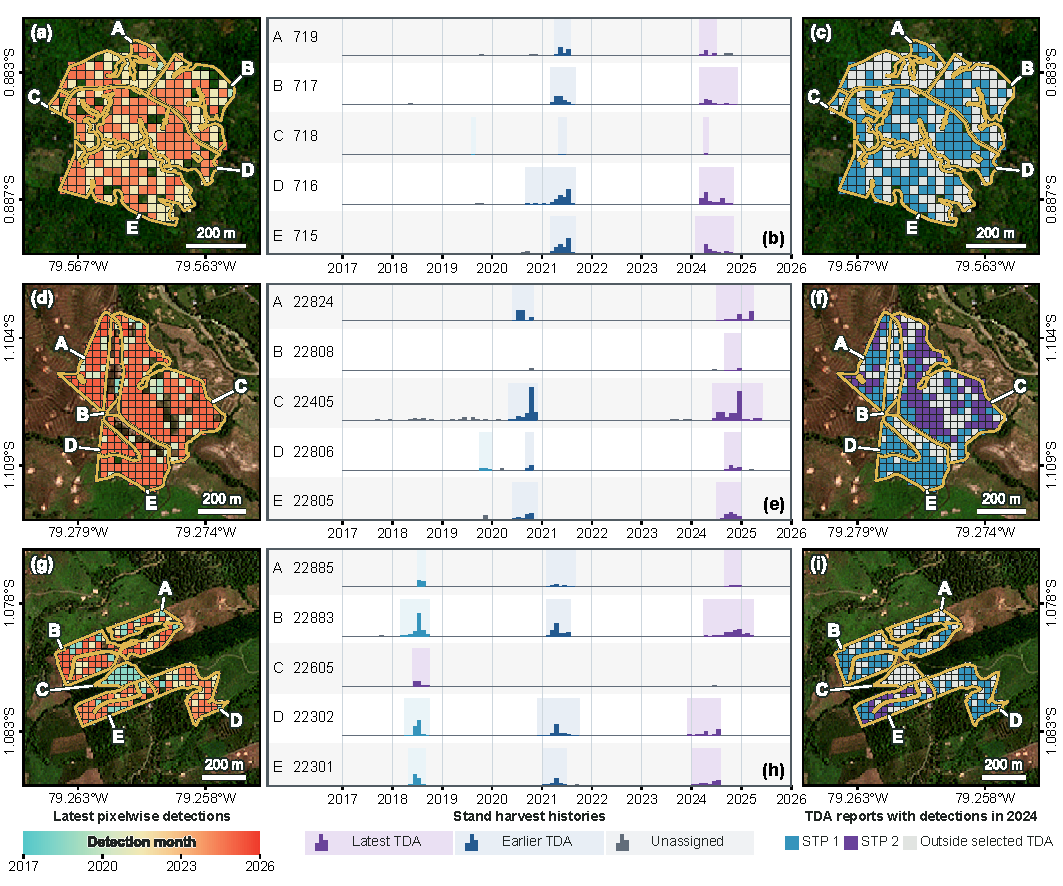
\includegraphics[width=\linewidth]{figures/fig06_stand_harvest_histories.pdf}
    \caption{Stand-level harvest histories and intra-event progression across three balsa neighbourhoods (March 2025 PlanetScope basemaps). (a,d,g) Latest pixelwise detection months (2017--2025). (b,e,h) Monthly detected-pixel counts (bars) and TDA event spans (shading; latest vs.\ earlier events). (c,f,i) Intra-event timing groups (STP~1 and STP~2) within complete TDA events containing 2024 detections. Letters (A--E) link stands across panels in each row.}
    \label{fig:harvest_mapping_stands}
\end{figure*}

Where harvesting progressed gradually across large management units, STP resolved distinct spatial felling stages within individual stand-level events without inflating stand harvest counts (Fig.~\ref{fig:harvest_mapping_stands}c,f,i). In Stand~22405, 109 of 156 pixels detected between June 2024 and May 2025 separated into two spatially coherent sub-blocks of 33 and 76 pixels centred in August and December 2024, respectively (Fig.~\ref{fig:harvest_mapping_stands}e,f). Similarly, in Stand~22301, pixels active between January and July 2024 partitioned into sub-blocks of 10 and 16 pixels centred in March and July 2024 (Fig.~\ref{fig:harvest_mapping_stands}h,i). Across the entire national inventory, STP identified significant spatial progression in 70 of the 2,125 size-eligible detected events, partitioning them into 142 intra-event timing groups.

\subsubsection{National harvesting hotspots, temporal pulses, and recurrence intervals}
\label{sec:mapping_national_recurrence}

Applying the framework across mainland Ecuador's balsa inventory (3,364 evaluable stands out of 3,498; 134 small polygons lacked 30~m grid-centre support) identified 6,303 stand-level harvest events across 2,931 stands during 2017--2025 (Fig.~\ref{fig:harvest_mapping_national}). Whereas 433 evaluable stands showed no harvest detection and 926 experienced a single harvest, 2,005 stands (59.6\%) underwent two or more harvests, confirming widespread multi-rotation management over the nine-year window.

\begin{figure*}[pos=!htbp]
    \centering
    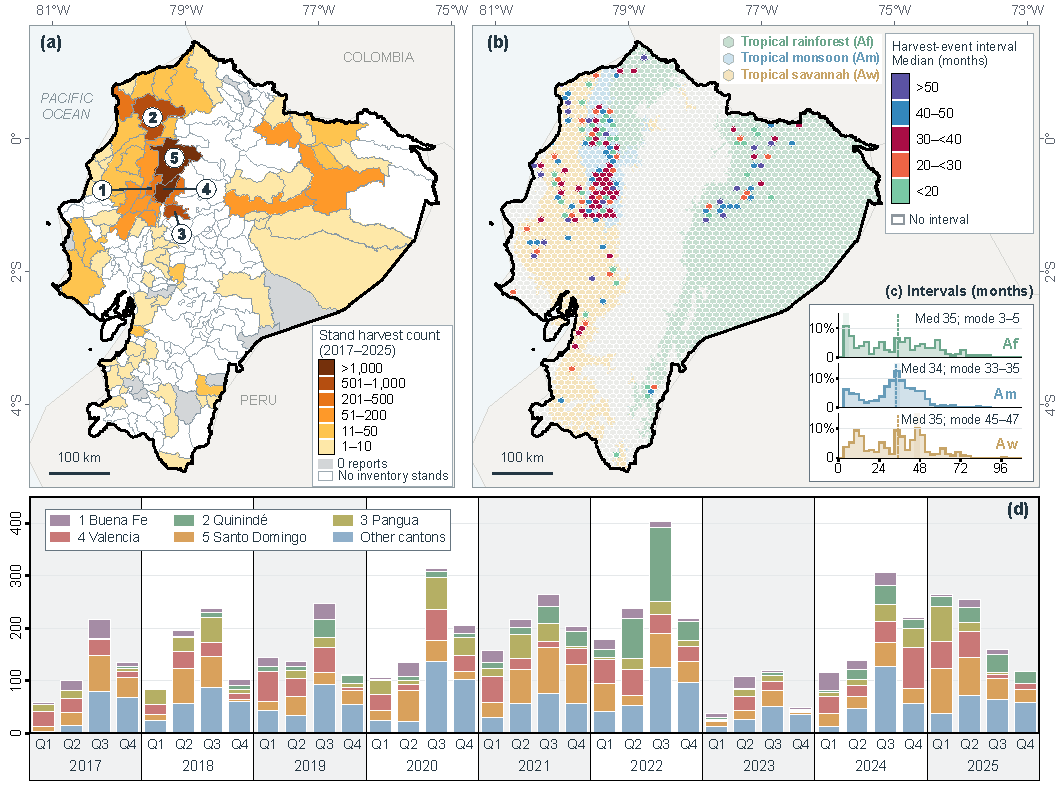
\includegraphics[width=\linewidth,height=0.74\textheight,keepaspectratio]{figures/fig07_national_harvest_patterns.pdf}
    \caption{National balsa harvest patterns in mainland Ecuador, 2017--2025. (a) Cumulative stand-level harvest counts by canton. (b) Modal inter-harvest intervals (3-month bins) in 10-km hexagons over K\"oppen--Geiger climate zones. (c) Inter-harvest interval distributions in Af, Am, and Aw climates (dashed lines: medians; purple bars: modal bins). (d) Quarterly stand-level harvest counts by canton.}
    \label{fig:harvest_mapping_national}
\end{figure*}

Cumulative harvest activity was strongly concentrated along the western coastal lowland and foothill plantation belt, delineating Ecuador's core production hotspots (Fig.~\ref{fig:harvest_mapping_national}a): five cantons---Santo Domingo (1,358 events), Valencia (1,076), Pangua (684), Quinind\'e (670), and Buena Fe (475)---accounted for 67.6\% (4,263/6,303) of all detected harvests nationwide. Temporally, harvesting exhibited a pronounced industry-wide cycle rather than a steady annual rate (Fig.~\ref{fig:harvest_mapping_national}d). Annual harvest events rose to a peak of 1,037 in 2022---culminating in the third quarter of 2022 with 403 events, including 141 in Quinind\'e alone---before dropping sharply to 315 in 2023 and rebounding to 781 in 2024 and 795 in 2025.

Across the 2,005 repeatedly harvested stands, consecutive stand-level events defined 3,372 inter-harvest intervals (measured between successive first-detection months), yielding a national median interval of 34 months (IQR: 22--43 months) and a dominant modal bin of 33--35 months (Fig.~\ref{fig:harvest_mapping_national}b,c). This national distribution was anchored by the tropical monsoon (Am) zone, which contained 84.8\% of all intervals ($n=2{,}861$), sharing the same 34-month median, 33--35 month mode, and a compact IQR of 24--42 months. Tropical savannah (Aw; $n=345$, 10.2\%) and tropical rainforest (Af; $n=150$, 4.4\%) stands exhibited nearly identical medians (35 months each) but wider dispersion and contrasting modal peaks: Aw shifted toward a longer modal bin of 45--47 months (IQR: 14--47 months), whereas the small Af sample peaked at 3--5 months alongside a broad IQR of 14.25--50 months.
